\documentclass{beamer}
\usepackage[utf8]{inputenc}

\usetheme{Madrid}
\usecolortheme{default}
\usepackage{amsmath}
\usepackage{amssymb,amsfonts,amsthm}
\usepackage{txfonts}
\usepackage{tkz-euclide}
\usepackage{listings}
\usepackage{adjustbox}
\usepackage{array}
\usepackage{tabularx}
\usepackage{gvv}
\usepackage{lmodern}
\usepackage{circuitikz}
\usepackage{tikz}
\usepackage{graphicx}

\setbeamertemplate{page number in head/foot}[totalframenumber]

\usepackage{tcolorbox}
\tcbuselibrary{minted,breakable,xparse,skins}



\definecolor{bg}{gray}{0.95}
\DeclareTCBListing{mintedbox}{O{}m!O{}}{%
  breakable=true,
  listing engine=minted,
  listing only,
  minted language=#2,
  minted style=default,
  minted options={%
    linenos,
    gobble=0,
    breaklines=true,
    breakafter=,,
    fontsize=\small,
    numbersep=8pt,
    #1},
  boxsep=0pt,
  left skip=0pt,
  right skip=0pt,
  left=25pt,
  right=0pt,
  top=3pt,
  bottom=3pt,
  arc=5pt,
  leftrule=0pt,
  rightrule=0pt,
  bottomrule=2pt,
  toprule=2pt,
  colback=bg,
  colframe=orange!70,
  enhanced,
  overlay={%
    \begin{tcbclipinterior}
    \fill[orange!20!white] (frame.south west) rectangle ([xshift=20pt]frame.north west);
    \end{tcbclipinterior}},
  #3,
}
\lstset{
    language=C,
    basicstyle=\ttfamily\small,
    keywordstyle=\color{blue},
    stringstyle=\color{orange},
    commentstyle=\color{green!60!black},
    numbers=left,
    numberstyle=\tiny\color{gray},
    breaklines=true,
    showstringspaces=false,
}
\title{1.1.25}
\date{26th March, 2026}
\author{Vishwambhar - EE25BTECH11025}

\begin{document}

\frame{\titlepage}
\begin{frame}{Question}
The state-space representation of a separately excited DC servo motor dynamics is given as:
\begin{align}
    \frac{d}{dt}\myvec{\omega\\i_a}=\myvec{-1&1\\-1&-10}\myvec{\omega\\i_a}+\myvec{0\\10}u
\end{align}
where $\omega$ is the speed, $i_a$ is the armature current, and $u$ is the armature voltage.\\
The transfer function $\frac{\omega\brak{s}}{u\brak{s}}$ 
\begin{enumerate}
    \item $\frac{10}{s^2+11s+11}$
    \item $\frac{1}{s^2+11s+11}$
    \item $\frac{10s+10}{s^2+11s+11}$
    \item $\frac{1}{s^2+s+1}$
\end{enumerate}
\end{frame}

\begin{frame}{Given}
\begin{align}
    \dot{\vec{x}}=A\vec{x}+\vec{b}u
\end{align}
where,
\begin{align}
    \vec{x}=\myvec{\omega\\i_a}\\
    A=\myvec{-1&1\\-1&-10}\\
    \vec{b}=\myvec{0\\10}
\end{align}
\end{frame}

\begin{frame}{Taking Laplace Transform}
\begin{align}
sX\brak{s}=AX\brak{s}+\vec{b}U\brak{s}\\
    \brak{sI-A}X\brak{S}=\vec{b}U\brak{s}\\
    X\brak{s}=\brak{sI-A}^{-1}+\vec{b}U\brak{s}
\end{align}
we only want $\omega$, so:
\begin{align}
    Y\brak{s}=\vec{c}\top X\brak{s}\\
    Y\brak{s}=\vec{c}\top \brak{sI-A}^{-1}bU\brak{s}
\end{align}
where,
\begin{align}
    c=\myvec{1\\0}
\end{align}
\end{frame}

\begin{frame}{Taking Laplace Transform}
\begin{align}
sX\brak{s}=AX\brak{s}+\vec{b}U\brak{s}\\
    \brak{sI-A}X\brak{S}=\vec{b}U\brak{s}\\
    X\brak{s}=\brak{sI-A}^{-1}+\vec{b}U\brak{s}
\end{align}
we only want $\omega$, so:
\begin{align}
    Y\brak{s}=\vec{c}\top X\brak{s}\\
    Y\brak{s}=\vec{c}\top \brak{sI-A}^{-1}bU\brak{s}
\end{align}
where,
\begin{align}
    c=\myvec{1\\0}
\end{align}
\end{frame}

\begin{frame}{Computing}
Final formula,
\begin{align}
    G\brak{s}=\frac{Y\brak{s}}{U\brak{s}}=\vec{c}\top\brak{sI-A}^{-1}b
\end{align}
Multiplying Everything,
\begin{align}
    \brak{sI-A}^{-1}b=\frac{1}{s^2+11s+11}\myvec{s+10&1\\-1&s+1}\myvec{0\\10}\\
    =\frac{1}{s^2+11s+11}\myvec{10\\10\brak{s+1}}
    G\brak{s}=\frac{10}{s^2+11s+11}
\end{align}
\end{frame}

\begin{frame}{Plot-Step Response}
    \begin{figure}
        \centering
        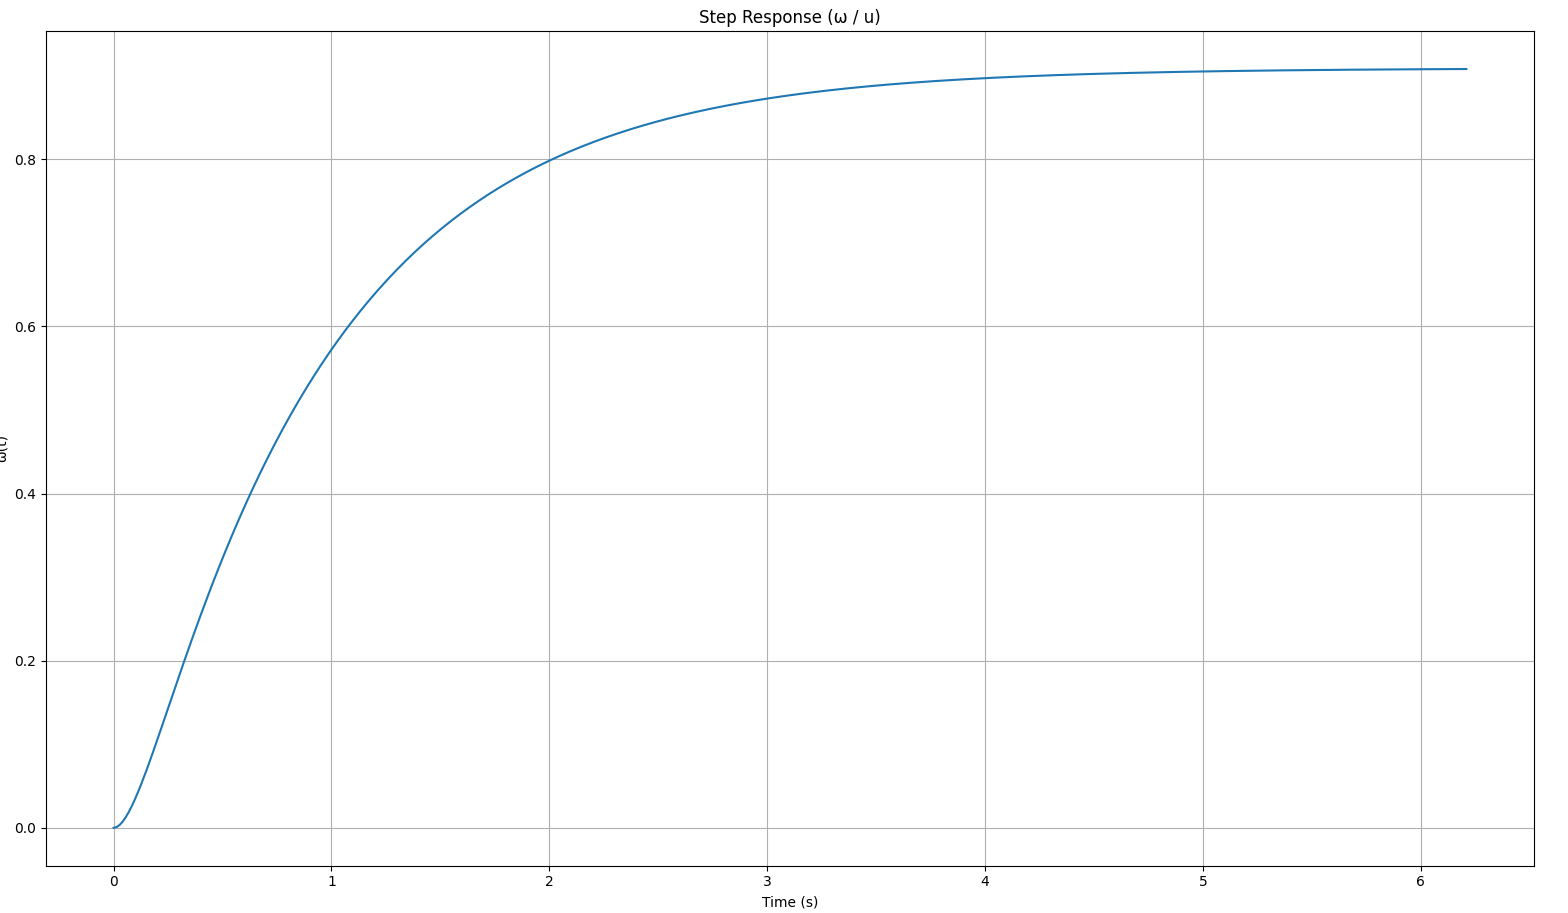
\includegraphics[width=1\columnwidth]{figs/step.png}
        \label{fig:fig}
    \end{figure}
\end{frame}

\begin{frame}{Plot-Impulse Response}
    \begin{figure}
        \centering
        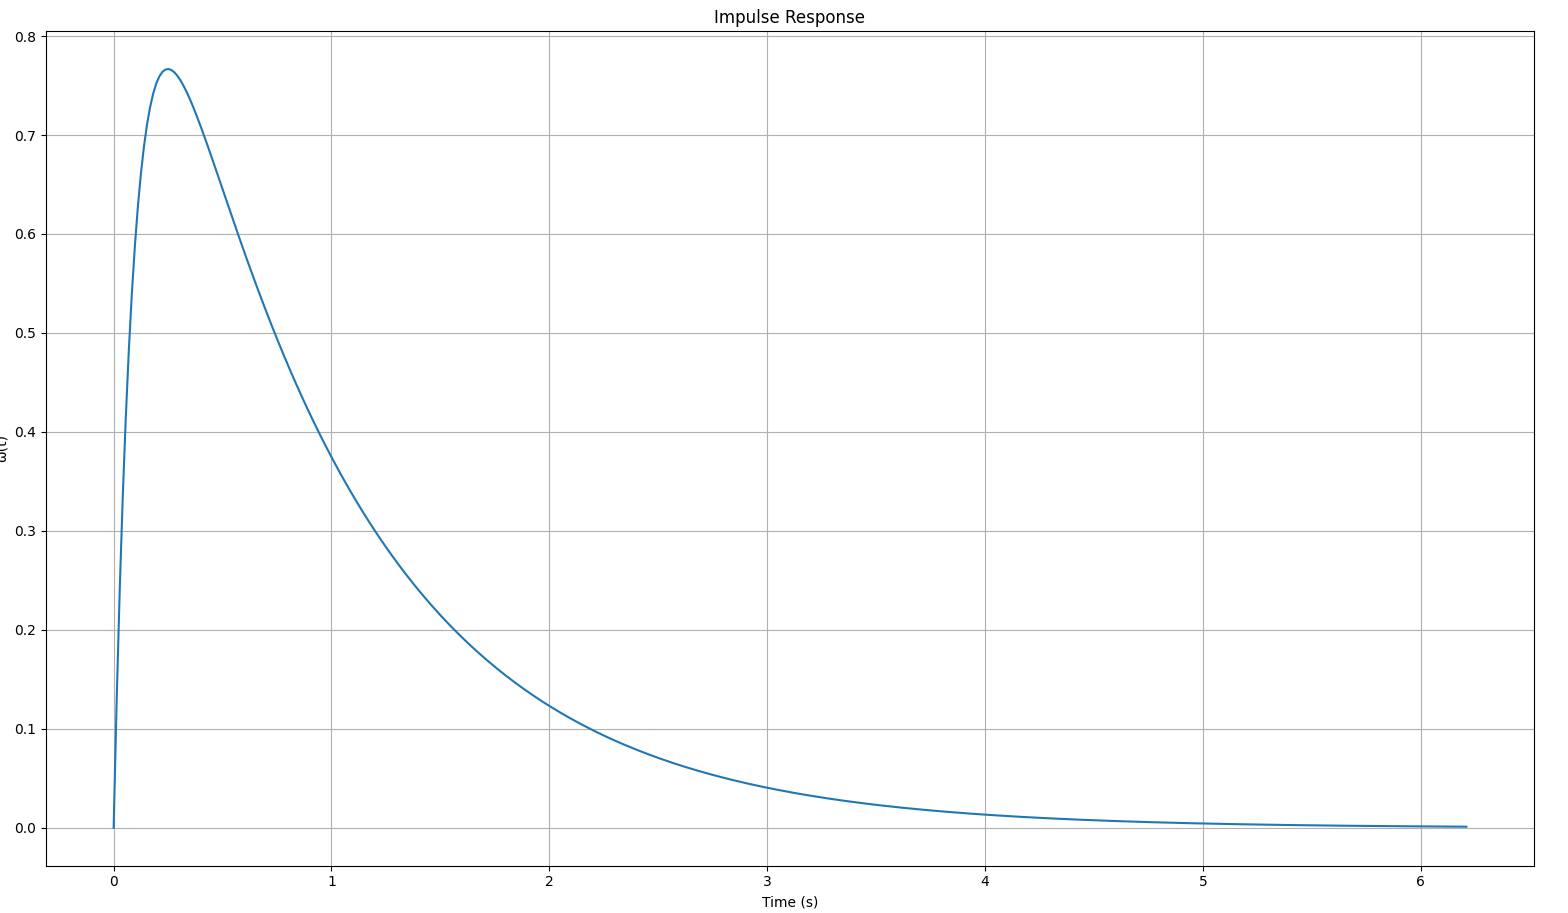
\includegraphics[width=1\columnwidth]{figs/impulse.png}
        \label{fig:fig}
    \end{figure}
\end{frame}

\begin{frame}{Plot-Sine Input(Bode)}
    \begin{figure}
        \centering
        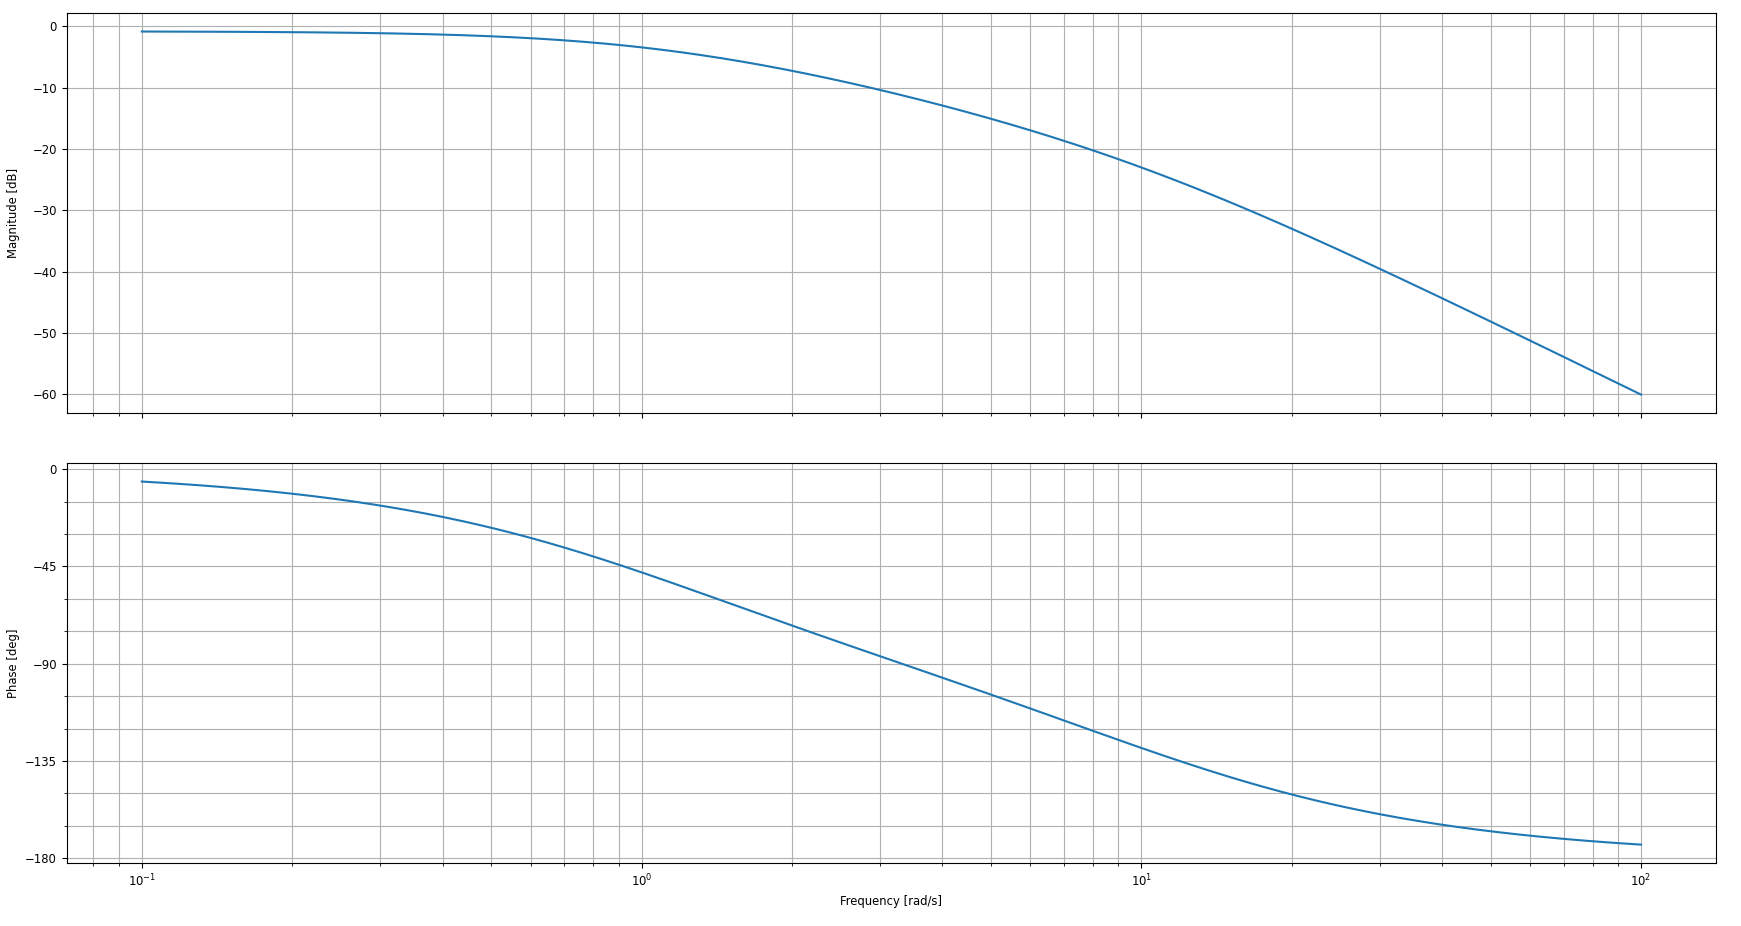
\includegraphics[width=1\columnwidth]{figs/bode.png}
        \label{fig:fig}
    \end{figure}
\end{frame}

\begin{frame}[fragile]
    \frametitle{Python Code}
    \begin{lstlisting}
import numpy as np
import matplotlib.pyplot as plt
import control as ctrl

# Define matrices
A = np.array([[-1, 1],
              [-1, -10]])
B = np.array([[0],
              [10]])
C = np.array([[1, 0]])
D = np.array([[0]])

sys_ss = ctrl.StateSpace(A, B, C, D)
sys_tf = ctrl.ss2tf(sys_ss)

print("Transfer Function:")
print(sys_tf)
    \end{lstlisting}
\end{frame}

\begin{frame}[fragile]
    \frametitle{Python Code}
    \begin{lstlisting}
# STEP RESPONSE
t, y = ctrl.step_response(sys_tf)
plt.figure()
plt.plot(t, y)
plt.title("Step Response (ω / u)")
plt.xlabel("Time (s)")
plt.ylabel("ω(t)")
plt.grid()
    \end{lstlisting}
\end{frame}

\begin{frame}[fragile]
    \frametitle{Python Code}
    \begin{lstlisting}
# IMPULSE RESPONSE
t, y = ctrl.impulse_response(sys_tf)
plt.figure()
plt.plot(t, y)
plt.title("Impulse Response")
plt.xlabel("Time (s)")
plt.ylabel("ω(t)")
plt.grid()

# BODE PLOT
plt.figure()
ctrl.bode(sys_tf, dB=True)

plt.show()
    \end{lstlisting}
\end{frame}
\end{document}